\documentclass[12pt,pdflatex]{elsarticle}

%%%%%%%%%%%%%%%%%%%%%%%%%%%%%%%%%%%%%%%%%%%%%%%%%%
%%%%%%%%%%%%%%%%%%%% PREAMBLE %%%%%%%%%%%%%%%%%%%%
%%%%%%%%%%%%%%%%%%%%%%%%%%%%%%%%%%%%%%%%%%%%%%%%%%


% -------------------- defaults -------------------- %
% load lots o' packages

% references
\usepackage{natbib}

% Fonts
\usepackage[default,oldstyle,scale=0.95]{opensans}
\usepackage[T1]{fontenc}
% \usepackage{ae}
% to colorize links in document. See color specification below
\usepackage[pdftex,hyperref,x11names]{xcolor}
% load the hyper-references package and set document info
\usepackage[pdftex]{hyperref}

% Generate some fake text
\usepackage{blindtext}

% layout control
\usepackage{geometry}
\geometry{verbose,tmargin=1.25in,bmargin=1.25in,lmargin=1.1in,rmargin=1.1in}
\usepackage{parallel}
\usepackage{parcolumns}
\usepackage{fancyhdr}

% math typesetting
\usepackage{array}
\usepackage{amsmath}
\usepackage{amssymb}
\usepackage{amsfonts}
\usepackage{relsize}
\usepackage{mathtools}
\usepackage{bm}
\usepackage[%
decimalsymbol=.,
digitsep=fullstop
]{siunitx}

% restricts float objects to be inserted before end of section
% creates float barriers
\usepackage[section]{placeins}

% tables
\usepackage{tabularx}
\usepackage{booktabs}
\usepackage{multicol}
\usepackage{multirow}
\usepackage{longtable}

% to adapt caption style
\usepackage[font={small},labelfont=bf]{caption}

% footnotes at bottom
\usepackage[bottom]{footmisc}

% to change enumeration symbols begin{enumerate}[(a)]
\usepackage{enumerate}

% to make enumerations and itemizations within paragraphs or
% lines. f.i. begin{inparaenum} for (a) is (b) and (c)
\usepackage{paralist}

% graphics stuff
\usepackage{subfigure}
\usepackage{graphicx}
\usepackage[space]{grffile} % allows us to specify directories that have spaces
\usepackage{placeins} % prevents floats from moving past a \FloatBarrier
\usepackage{tikz}
\usetikzlibrary{arrows, positioning, shapes.geometric,calc}
\usepackage{rotating}

% Spacing
\usepackage[doublespacing]{setspace}

% Add some colors
\definecolor{red1}{RGB}{253,219,199}
\definecolor{red2}{RGB}{244,165,130}
\definecolor{red3}{RGB}{178,24,43}

\definecolor{green1}{RGB}{229,245,224}
\definecolor{green2}{RGB}{161,217,155}
\definecolor{green3}{RGB}{49,163,84}

\definecolor{blue0}{RGB}{255,247,251}
\definecolor{blue1}{RGB}{222,235,247}
\definecolor{blue2}{RGB}{158,202,225}
\definecolor{blue3}{RGB}{49,130,189}
\definecolor{blue4}{RGB}{4,90,141}

\definecolor{purple1}{RGB}{191,211,230}
\definecolor{purple2}{RGB}{140,150,198}
\definecolor{purple3}{RGB}{140,107,177}

\definecolor{brown1}{RGB}{246,232,195}
\definecolor{brown2}{RGB}{223,194,125}
\definecolor{brown3}{RGB}{191,129,45}

\definecolor{cyan1}{RGB}{224,255,255}
\definecolor{cyan2}{RGB}{0,200,200}
\definecolor{cyan3}{RGB}{0,139,139}

% -------------------------------------------------- %


% -------------------- page template -------------------- %

\setlength{\headheight}{15pt}
\setlength{\headsep}{20pt}
\pagestyle{fancyplain}

\fancyhf{}

\lhead{\fancyplain{}{}}
\chead{\fancyplain{}{Networks \& State Preferences}}
\rhead{\fancyplain{}{}}
\rfoot{\fancyplain{}{\thepage}}

% ----------------------------------------------- %


% -------------------- customizations -------------------- %

% easy commands for number propers
\newcommand{\bl}[1]{{\mathbf #1}}
\newcommand{\first}{$1^{\text{st}}$}
\newcommand{\second}{$2^{\text{nd}}$}
\newcommand{\third}{$3^{\text{rd}}$}
\newcommand{\nth}[1]{${#1}^{\text{th}}$}

% easy command for boldface math symbols
\newcommand{\mbs}[1]{\boldsymbol{#1}}

% command for R package font
\newcommand{\pkg}[1]{{\fontseries{b}\selectfont #1}}

% approx iid
\newcommand\simiid{\stackrel{\mathclap{\normalfont\mbox{\tiny{iid}}}}{\sim}}

% -------------------------------------------------------- %

%%%%%%%%%%%%%%%%%%%%%%%%%%%%%%%%%%%%%%%%%%%%%%%%%%
%%%%%%%%%%%%%%%%%%%% DOCUMENT %%%%%%%%%%%%%%%%%%%%
%%%%%%%%%%%%%%%%%%%%%%%%%%%%%%%%%%%%%%%%%%%%%%%%%%

% remove silly elsevier preprint note
\makeatletter
\def\ps@pprintTitle{%
 \let\@oddhead\@empty
 \let\@evenhead\@empty
 \def\@oddfoot{}%
 \let\@evenfoot\@oddfoot}

\makeatother

\usepackage{etoolbox}
\makeatletter
    \patchcmd{\@author}{\global\let\@fnmark\@empty}{\global\let\@fnmark\@empty\global\let\@corref\@empty}{}{\@latex@error{Failed to patch \string\@author for \string\@corref reset}}
\makeatother

\journal{}

\begin{document}

% saying hello ----------------------------------------------- %
\thispagestyle{empty}
\begin{frontmatter}

% \title{A Network Approach to Measuring State Preferences}
\title{A Network Approach to Measuring State Preferences \tnoteref{t1}}
\tnotetext[label1]{Author order is alphabetical.}

\tnotetext[t1]{We would like to thank comments from discussants and audience members at the International Studies Association and Midwest Political Science Association Conferences as well as participants from the Government Speaker Series at the University of Essex. We are also grateful for comments from three anonymous reviewers who provided thoughtful insight to help us improve our paper.}

\author[strath]{Max Gallop}
\ead{max.gallop@strath.ac.uk}
\author[msu]{Shahryar Minhas\corref{cor1}}
\ead{minhassh@msu.edu}
%
\cortext[cor1]{Corresponding author}
%
\address[strath]{Departments of Political Science, University of Strathclyde}
\address[msu]{Department of Political Science, Michigan State University}

\begin{abstract}
\singlespacing{State preferences play an important role in international politics. Unfortunately, actually observing and measuring these preferences is impossible. In general, scholars have tried to infer preferences using either UN voting or alliance behavior. The two most notable measures of state preferences that have flowed from this research area are ideal points (Bailey et al., 2017) and S-scores (Signorino \& Ritter, 1999). The basis of both these models is a spatial weighting scheme that has proven useful but discounts higher-order effects that might be present in relational data structures such as UN voting and alliances. We begin by arguing that both alliances and UN voting are simply examples of the multiple layers upon which states interact with one another. To estimate a measure of state preferences, we utilize a tensor decomposition model that provides a reduced-rank approximation of the main patterns across the layers. Our new measure of preferences plausibly describes important state relations, and yields important insights on the relationship between preferences, democracy, and international conflict. Additionally, we show that a model of conflict using this measure of state preferences decisively outperforms models using extant measures when it comes to predicting conflict in an out-of-sample context.}
\end{abstract}

\end{frontmatter}
% ----------------------------------------------- %

\newpage\setcounter{page}{1}


\section*{Why we care about preferences}

Understanding state interactions in the realm of international politics necessitates some knowledge of states' foreign policy preferences vis-\`{a}-vis each other.  We can consider each state to have a preferred policy outcome on each possible issue that might arise in international relations. We can conceive of these preferred outcomes as an ideal point in multidimensional space. Given the fact that many issues in international politics are related, we can represent these preferences in far fewer dimensions than there are issues in international politics. These preferences will also change over time. When states have similar preferences on an issue, they will be more likely to collaborate to achieve their joint preference on that issue, and more generally states with similar foreign policy preferences will be cooperative in a larger proportion of their interactions. States with similar preferences are also unlikely to be involved in violent disputes with each other because the policy benefits of these disputes are unlikely to surpass the cost of fighting. Conversely, when states have highly dissimilar foreign policy preferences, cooperation will be difficult and violence will be more common. Unfortunately, while we have abundant data to measure the strength of states' economies, the volume of trade between states, or even their military power, it is much more difficult to measure the similarity of states' preferences, because as with many social and political constructs they cannot be observed directly.

Effectively measuring state preferences would yield scholars a number of benefits. A number of formal theories of international relations require measures of preferences to be tested: the expected utility theory proffered by \citep{buenodemesquita:1983} has similarity of preferences as an important input. Further attempts to expand studies of crisis bargaining to include mediation \citep{kydd:2003}, coalitional dynamics \citep{wolford:2014}, or the possibility of additional disputants \citep{gallop:2017} require a measure of state preferences in order to predict whether war will be the result of bargaining failure. Preference similarity have been used in empirical studies predicting bilateral trade, foreign aid, stability of international institutions and the incidence of conflict \citep{derouen:heo:2004, stone:2004, gartzke:2007, kastner:2007, braumoeller:2008}.

A substantive theoretical reason for why we need a good measure of preference similarity is to correctly understand the democratic peace. It is difficult to entangle whether democracies avoid war with other democracies because of the intrinsic nature of democracy, or simply because they appear to share similar ends. \citet{farber:gowa:1995} argue that democracies were only peaceful during the Cold War period because they had similar preferences and alliance structures. Similarly, \citet{gartzke:1998} argues that dissimilar preferences are a necessary condition for conflict. \citet{oneal:russett:1999e} respond by arguing that democracy has both a direct inhibiting effect on conflict, and an indirect one through influencing state preferences.\footnote{\citet{gartzke:2000} argued that even though democracies might have similar preferences, the residual of preferences from democracy explains conflict much better than the residual of democracy from preferences.} While there has been some impressive development with measures of preferences in recent years, a more accurate measure is essential to disentangle the extent to which peace is the product of shared preferences, and the extent to which institutions and norms are driving peace.

Much of the extant literature has focused on estimating preferences similarity by utilizing spatial weighting models on either alliance behavior or United Nations (UN) voting scores. These approaches have proven to be useful but there are two reasons to desire a different approach. First, alliances are rare and voting together in the UN is very common, so, by only focusing on the direct dyadic behavior, we risk mischaracterizing important relationships. Second, we would expect a better understanding of state preferences to help us predict state behavior, but as we show in Figure \ref{fig:rocShitty} adding measures of  preference similarity to a traditional model of interstate disputes yields relatively scant increases in terms of predictive ability.

\begin{figure}[ht]
	\centering
	\begin{tabular}{cc}
	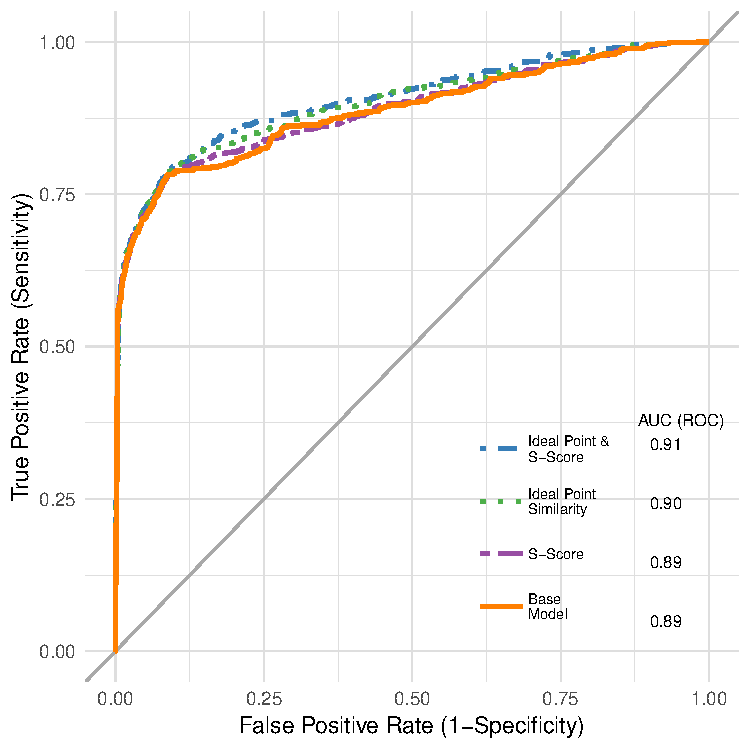
\includegraphics[width=.5\textwidth]{roc_outSample_noLatAngle.pdf} &
	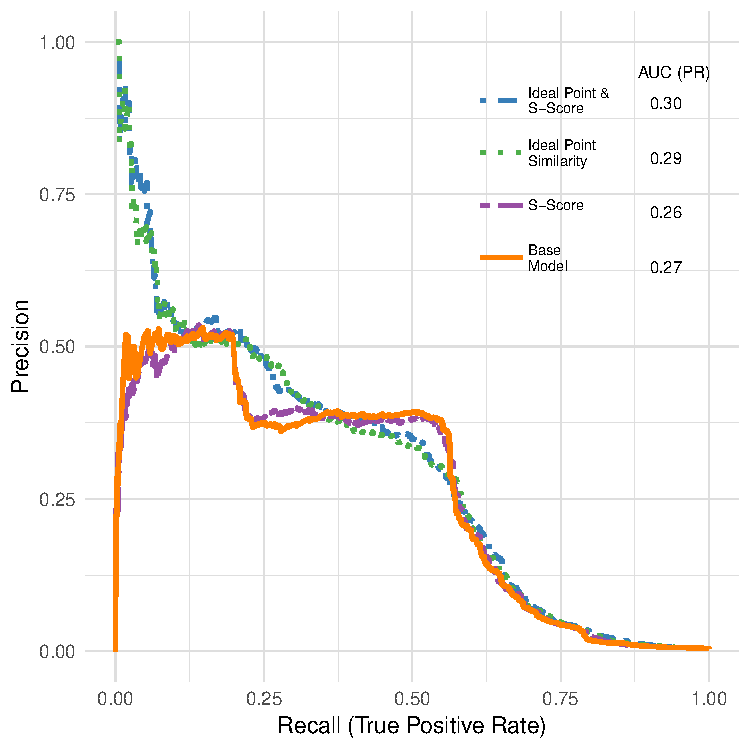
\includegraphics[width=.5\textwidth]{rocPr_outSample_noLatAngle.pdf}
	\end{tabular}
	\caption{Assessments of out-of-sample predictive performance of Militarized Interstate Disputes using ROC curves and PR curves. AUC statistics are provided as well for both curves.}
	\label{fig:rocShitty}
\end{figure}

We can improve on these measures of preference similarity using the same raw material by acknowledging that both alliance membership and UN voting are layers of relationships that takes place simultaneously and in an interdependent context. Specifically, these relations between states constitute a multilayer network, in which the various layers correspond to different ways states are interacting with one another at a given time point. A bevy of research has shown that accounting for network structure necessitates an approach that can account for the indirect relations states share. As such, we make two contributions to the existing literature on state preferences. We utilize a multilinear tensor regression that enables us to measure how dependent actions of a particular dyad are across layers and time. We show that our revised approach of measuring state preference similarity both better characterizes relationships that have had counterintuitive results, and this measure greatly enhances our ability to predict instances of conflict.


\section*{Sources of Preference Measures: Alliance Portfolios and UN Voting}

Given that we cannot directly observe state preferences, scholars have attempted to estimate preferences using two main behavioral indicators: who states choose to ally with and how states vote at the UN. The idea behind alliance portfolio measures is that we can infer a state's foreign policy by looking at the states they choose to align with. In the extreme case, if two states have all of the same allies, it is likely that their foreign policy goals are quite similar. Conversely, if all allies of one state are not allied to another, and vice versa, our best guess is that these states would have different aims and desires in foreign policy. \citet{buenodemesquita:lalman:2008} encapsulate the logic by noting ``alliance commitments reflect a nation's position on major international issues''. Measures of alliance behavior do, however, suffer from the fact that these measures are largely static and sparsely occurring. Formal alliances are relatively constant over time, whereas in many cases state preferences will be more fluid, and therefore these scores will be at best a lagging indicator of preferences. Furthermore, \citet{hage:2011} shows that the rarity of links creates an artificial similarity of alliance portfolios.

We also have a relatively large corpus of behavioral information in UN Voting Records. The cost of voting in the UN is low, and so, scholars argue that measures of affinity based on UN voting are relatively representative of the underlying distribution of preferences \citep{gartzke:1998}. This is especially fortuitous because the methodology of inferring preferences from voting in a legislature is advanced. A few issues with these measures are that the potential benefit of winning UN votes is low, and so states might have incentives to vote against their preference as they are not costly signals, and the distribution of UN voting is prone to large supermajorities of the type rarely seen in ``ordinary" legislatures.

\subsection*{S-Scores \& Alliance Portfolios}

 One of the first measures used to measure preference similarity based on alliance portfolios is Kendall's $\tau_{B}$ \citep{buenodemesquita:lalman:2008}. This is operationalized as:

 \begin{equation}
	 \tau_{B} = \frac{n_{c} - n_{d}}{\sqrt{(n_{0} - n_{1})(n_{0} - n_{2})}}
 \end{equation}

 \noindent where $n_{c}$ is the number of pairs where both actor $i$ and $j$ have the same rank ordering (for example both the United Kingdom and the United States are more closely allied to Israel than to Iran), $n_{d}$ is the number of pairs where they have discordant rankings (the United States is more closely allied to Saudi Arabia than to Russia, Syria is more closely allied to Russia than to Saudi Arabia). The denominator attempts to adjust the total number of pairs with the number of ties: $n_{0}$ is the total number of pairs ($n(n-1)/2$), $n_{1}, n_{2}$ are measures for ties in both $i$ and $j$'s rankings respectively.

\citet{signorino:ritter:1999} convincingly point to flaws in this measure, notably its focus on rank-ordering as applied to a context where we instead care mostly about the presence or absence of an alliance. Additionally, adding more strategically irrelevant states will create artificially high $\tau_{B}$ statistics. Thus, Signorino and Ritter introduce the S-score, which has since been the most widely used alliance similarity measure.\footnote{\citet{bennett:rupert:2003} also find a stronger relationship between theoretical predictions and results when using S-scores than when using $\tau_{B}$.} The equation for the S-score is:

\begin{equation}
	S(P^i, P^j, W, L) = 1 - 2w_k \frac{d(P^i, P^j, W, L)}{d^{\text{max}}(W,L)}
\end{equation}

\noindent here $P^{i}$ and $P^{j}$ are vectors of length $N$, showing the relation that states $i$ and $j$ have to each of the $N$ states (including themselves).\footnote{The entries in $P^{i}$ could be binary, or they could be allowed to give more weight to stronger relationships, in the case of alliances they generally take on values between 0 and 3, with 0 denoting no alliance, and 1 an entente, 2 a non-aggression pact, and 3 a mutual defense pact.} $W$ is a vector of weights (normalized to sum to $1$), allowing a scholar to ascribe higher (lower) values for more (less) important states. For example, the weights matrix can be adjusted so that relations with China play a larger role in two states' similarity score than relations with a less globally relevant country. $d(P^i, P^j, W, L)$ is the distance between portfolio $i$ ($P^i$) and portfolio $j$ ($P^j$) based on the vector of weights $W$ and the scoring rule $L$. If using an absolute distance scoring rule, then $d(P^{i}, P^{j}, W, L) = \sum_{k = 1}^{N} \frac{w_{k}}{\Delta^{\text{max}_{k}}} |p^{i_{k}} - p^{j_{k}}|$.

In other words, we would calculate the distance between the two portfolios by looking at the absolute distance between each item in the portfolio ($p^i_{k}$ for state $i$'s relationship with state $k$) adjusted by the weight given to this relationship ($w_{k}$) and then normalized by $\Delta^{\text{max}_{k}}$, the maximum possible difference between $p^{i_{k}}$ and $p^{j_{k}}$. $d^{\text{max}}(W,L)$ is the largest distance between portfolios observed in the policy space, so this means that states at the maximum observed distance will have an S-score of $-1$, and those with identical portfolios will have an S-score of $1$. For the weight matrix, generally, analysts have used S-scores calculated with a weight matrix of ones--giving each potential ally equal weight--though the other plausible choice would be to weight states by importance, for example using their share of world military capability, as calculated by \citet{singer:small:1995}.

In recent years, some scholars have started to argue that forming and maintaining alliances are not independent dyadic phenomena, but are rather part of an interdependent network (or series of networks). \citet{warren:2010} illustrates how extra-dyadic factors matter for alliance formation, in particular alliances with allies of your allies (and enemies of your enemies) are more likely. Further investigation uncovered that other network effects such as popularity and 2-stars can drive alliance formation as well \citep{cranmer:etal:2015}. The strategic nature of states when they form alliance ties leads to interdependence in the alliance network, as states seek to ensure their strength and security as efficiently as possible, privileging ties that complete triangles, and paying attention to the decreasing returns of additional alliances \citep{cranmer:etal:2012}. Later, \citet{warren:2016} demonstrated not only are network effects (like preferential attachment, density, and transitivity) important in the generation of the alliance network, but the alliance network and the conflict network are mutually constitutive. Similarly, \citet{kinne:bunte:2018} uncover links between the network of defense cooperation, and the network of bilateral loans, as states strategically loans to exert policy influence on other states, and strategically formed communities of defense cooperation in order to enhance the power and independence of its members.

\subsection*{Ideal Points \& UN Voting Similarity}

An advantage of utilizing UN General Assembly Voting, is that it allows the field to take advantage of methodological advances that have been made in the study of legislatures \citep{poole:rosenthal:1985}. \citet{bailey:etal:2015} do so by using an Item Response Theory model on UNGA voting. This model places states on a unidimensional latent preference space based on their voting behavior. The assumption of this model is that states' votes on a resolution are a function of states' ideal points, characteristics of the vote, and random error. In particular, for each bill $v$, a state's vote will be based on the latent variable $Z_{itv}$, representing the preference of state $i$, on vote $v$, at time $t$, defined such that:

\begin{equation}
	Z_{itv} = \beta_{v}\theta_{it} + \epsilon_{iv}
\end{equation}

\noindent Where $\beta_{v}$ is the discrimination factor of bill $v$, determining whether states with high ideal points will vote yes (if $\beta_{v}$ is negative) or no (positive). $\theta_{it}$ is state $i$'s ideal point at time $t$, and $\epsilon_{iv}$ is actor and bill specific error. Of course, we do not observe the latent variable, and only observe the outcome $Y_{itv}$, which will either be yes, no, or abstention. The model creates a pair of cutpoints $\gamma_{1v}$ and $\gamma_{2v}$ in the preference space, such that  if $Z_{itv} < \gamma_{1v}$, $Y_{itv} = \text{Yes}$, if $Z_{itv} > \gamma_{2v}, Y_{itv} = \text{No}$ and otherwise abstain. This allows the model to use observed vote outcomes in order to determine each states' ideal point in each year.

The authors specifically fix the parameters $\gamma_{1v}$ and $\gamma_{2v}$ such that the same bill will have the same value in different years, and they standardize and normalize $\theta$. They also use $\theta_{it-1}$ as a prior on $\theta_{it}$. With these constraints, they solve for the ideal points using a Metropolis Hastings Markov Chain Monte Carlo (MCMC).

Both methods relying on UN data, and those relying on alliances have difficulties distinguishing within '0's and '1's. For example, if we know two states are allies, we have reason to believe they have similar preferences, but if we know they are not allies, it is not clear whether they are enemies or they are indifferent -- the United States is ``not-allies" with both Bhutan and North Korea for example. As of 2012, using the Correlates of War projects alliance data, only about 1/8th of all dyads were between countries with any sort of alliance. Similarly, with UN voting, so many UN votes contain super-majorities and states vote together a huge proportion of the time. If we only look at yes and no votes in the UN general assembly, the median pair of states has voted together about 96\% of the time. If we include abstentions,  they have voted together 86\% of the time. So when two states vote together it is hard to distinguish between states voting together because of similar preferences, or just preferences that are not radically dissimilar. Both S-scores and Item Response theory succeed in adding granularity and nuance to these rough measures, but they are both limited by focusing only on a relationship between two states.

We can see the potential issues of focusing only on direct relations when we view how these two measures of preference treat relations over the Korean peninsula. If we take China, North Korea, South Korea, and the United States, we would expect the United States and South Korea to have preferences that are similar to each other and dissimilar from China and North Korea (and vice versa). Yet, if we look at extant measures of preferences (as of 2012), as depicted in Figure \ref{korean:prefs}, they do not seem to effectively characterize this relationship. S-scores based on alliance portfolios posit that China and the two Koreas are closely clustered, with the United States distant from all three, while ideal point distances put China's relationship with South Korea on par with its relationship with North Korea. Now it could be that these measures are producing a novel, counterintuitive, result, but given the failures of extant preference measures to add much to predictive models of conflict, one might be skeptical.

\begin{figure}[ht]
	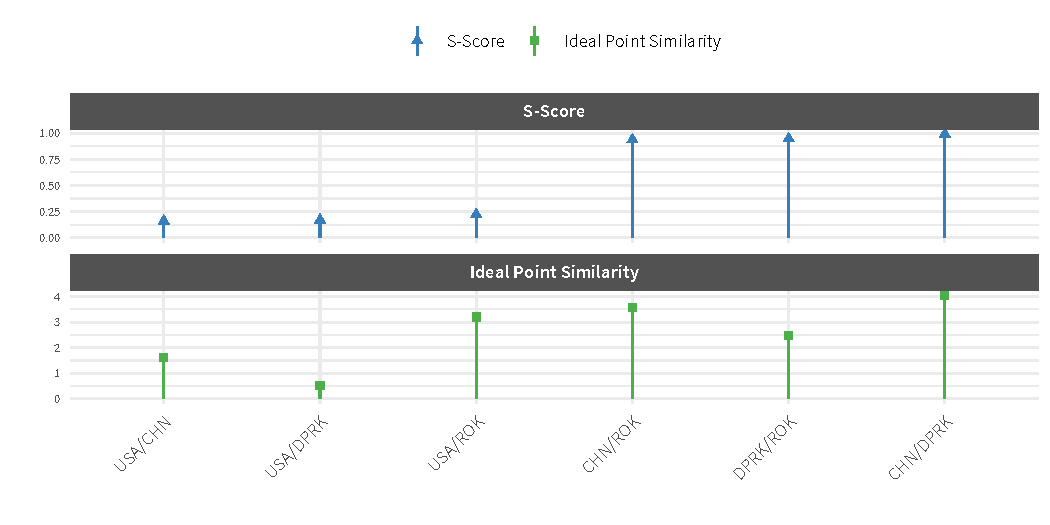
\includegraphics[width=1\textwidth]{idPtScoreViz.pdf}
	\caption{Visualization of ideal point distance and S-score relationships between China (CHN), North Korea (DPRK), South Korea (ROK), and the United States (USA) in 2012. Within each panel a higher score denotes that the countries have a more positive relationship.}
	\label{korean:prefs}
\end{figure}

The sources of these surprising results become more clear when looking at the data on which they are based. In 2012, according to the Correlates of War, North Korea only had 3 alliances -- a non-aggression pact with the South, and alliances with Russia and China. Similarly, South Korea's only alliances were that non-aggression pact, and an alliance with the United States. Given the United States' many other allies, there was much more divergence between their alliance portfolio and South Korea's, than there was between the two Koreas' portfolios \citep{gibler:sarkees:2004}. Similarly, when looking at voting patterns at the UN, South Korea voted 50\% of the time with the US, 63\% of the time with North Korea, and 70\% of the time with China.

Even using this data, we can better approximate state preferences when we treat alliances and UN voting as relational data. When it comes to alliance behavior, the fact that North Korea was allies with China and Russia, and South Korea with the United States could give us additional information, because the alliance behaviors of countries such as the United States and China are so divergent. When looking at voting patterns at the UN, the need for a relational approach is even more apparent. While South Korea only voted with the US 50\% of the time at the UN, this was in the top 15\% of all countries in terms of voting with the US, whereas South Korea was in the bottom 20\% in terms of the proportion of time voting with China.

We thus argue that two changes can substantially improve measures of state preferences. First, both alliances and UN voting contain information about state foreign policy preferences, and given the limits of this information, we should find a way to use both. Second, by using network techniques and treating this data as relational data, we can wring more information from the stone, and get both a more nuanced, and more accurate view of state affinity and state preferences.

\section*{Synthesizing Measures of State Preference}

The approach that we introduce here to measure state preference similarity starts by assuming that both UN voting and alliance relationships are sources of information on how states relate to one another on the international stage. By accounting for the multiple layers upon which states interact with one another we can synthesize a better measure of preference similarity than if we relied on any one measure alone. The idea of using multiple metrics to get a better handle on preferences is not new, in fact, Signorino and Ritter suggested it in introducing S-scores, which were designed to allow for aggregation of similarity on multiple dimensions (such as alliances and UN voting). The downside of this extant approach, however, is that it does not account for structural patterns that we often see in relational data.

Relational data is composed of observations between pairs of actors, or dyads. For both alliance relationships and UN voting, we are able to observe how the actors in the international system interact with one another across time. This system of interactions taken in its totality defines a network, and within these types of structures a bevy of research has shown that we need methods that go beyond assuming that interactions are taking place between just two actors in a vacuum \citep{wasserman:faust:1994,snijders:nowicki:1997,minhas:etal:2019}. As such we reformulate the problem of determining state preferences in terms of a network analysis. The goal of our approach is summarized in Figure~\ref{fig:tensViz}. In the top row, we represent UN voting and alliance patterns at time $t$ as a pair of adjacency matrices that form an evolving multiplex network.\footnote{The approach that we describe here can be generalized to a multiplex with more than two dimensions.} Our goal is to extract a lower dimensional representation of this system, such that the output is a series of $n \times n$ matrices, where $n$ represents the number of actors and in which the cross-sections denote our estimates of the preference similarities between countries.

\begin{figure}[ht]
	\centering
	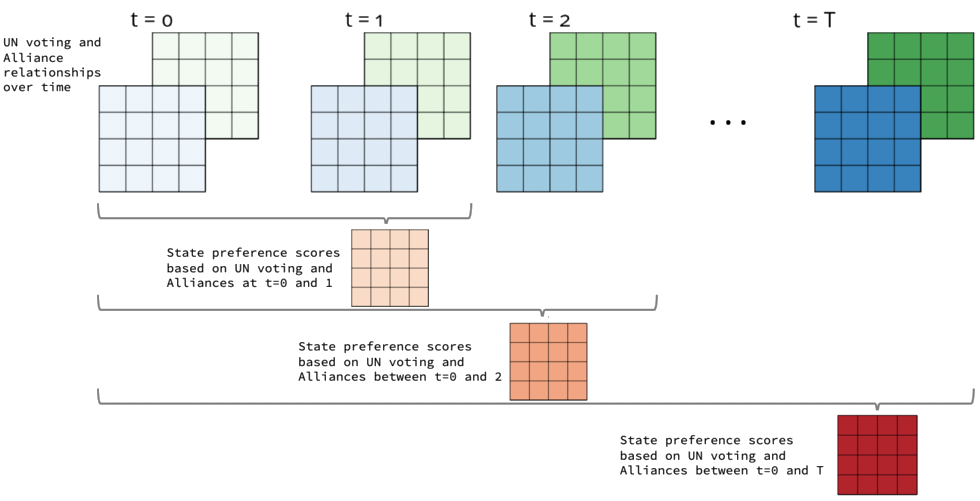
\includegraphics[width=1\textwidth]{tensor_viz.png}
	\caption{The green and blue colors represent different relational measures and darker shading indicates later time periods. Our goal is to reduce the patterns found across those layers of relationships into a single measure.}
	\label{fig:tensViz}
\end{figure}

We generate these estimates through a multilinear tensor regression model that combines information across networks and time to measure how dependent the actions of a particular state are on another \citep{hoff:2015,minhas:etal:2016}. By incorporating information from multiple measures through a network perspective, we show that our approach improves on alternative measurements of state preference when it comes to predicting and explaining interstate conflict.

\subsection*{Multilinear Tensor Regression}

Our goal here is to measure a concept that is not directly observable. This is a problem that is very familiar in political science and a number of techniques based on measurement models have been developed to study political ideology \citep{martin:quinn:2002,konig:etal:2013}, human rights abuses \citep{fariss:2014}, and judicial independence \citep{linzer:staton:2015}. Obviously, the ideal points measure developed by \citet{bailey:etal:2015} also follows in this growing practice of extracting unobserved information via a spatial weighting scheme. Here we build on this general goal by developing a measurement of how a state relates to other states in a network context. Substantively, this goal is no different than how others have sought to find simpler representations of legislators and bills \citep{poole:rosenthal:1985,clinton:etal:2004}, but the key difference from shifting to the network is the recognition that we can better understand the relations between a pair of states by understanding how they relate to others in the international system.

We represent relational data that is longitudinal as an array $\bl Y = \{\bl Y_t : t = 1, \ldots T\}$, with each $\bl Y_t$ representing the actions between countries in a given year $t$. A cross-sectional entry such as $y_{i,j,v,t}$ from $\bl Y$ denotes an interaction that occurred between actors $i$ and $j$ at time $t$ across variable $v$. These series of matrices can be assembled in a tensor, $\bl Y$, which we use to represent actors interacting over time across multiple measures. Specifically, $\bl Y$ will have dimensions $n \times n \times p \times T$, where $n$ corresponds to the number of countries, $p$ to the number of variables (i.e., relational measures), and $T$ to the number of time periods.

The information contained in this set of matrices can also be represented as a vector, where $(\mathbf y_t)$ represents a time series of vectors representing the dyadic interactions across multiple variables for $n$ countries through the period $t = 1, \ldots, T$. Transforming the data in this way enables us to think of what we are modeling in an explicitly time series context, where the evolution of multiple series is a function of their past behavior. Modeling such processes can often be accomplished using a vector autoregression (VAR) framework:

\begin{eqnarray}
	\bl y_t &=& { \Theta \bl y_{t-1} +\bl e_t}\\
	E[\bl e_t] &=& 0 \\
	E[\bl e_t \bl e^T_s] &=& \begin{cases}   \Sigma &\mbox{if } t=s, \\ 0 &\mbox{otherwise}\end{cases}
\end{eqnarray}

However, given the data requirements of estimating $\Theta$,\footnote{$\Theta$ has $n^4$ entries.} \citet{hoff:2015} employs a bilinear regression model such that the regression matrix is given by $ \Theta = \bl B \otimes \bl A$.\footnote{$\otimes$ is the Kronecker product.} As a result, we obtain the following basic specification: $\bl Y_t = \bl A \bl Y_{t-1}\bl B^T$. An alternative approach to this tensor decomposition could have involved the usage of a network latent variable model scheme. The key difference between those models and this tensor approach is that in the former we are projecting the relations between actors onto lower a dimensional space, where similarity in orientation indicates that actors are more likely to have similar dependence patterns. In the context of this model, $\bl A$ and $\bl B$ are $n \times n$ matrices of regressions coefficients, where each cross-sectional entry measures the level of dependence between the sending relationships of a particular actor and  $B$ the receiving relationships.

The tensor regression problem can also be written somewhat more simply in tensor form, where it is clearer that we are essentially regressing the relational tensor $\bl Y_t$ from time $t$ on the tensor $\bl Y_{t-1}$ from time $t-1$:

\begin{equation}
	\bl Y = \bl Y_{t-1} \boldsymbol{\times} \{ \bl A, \bl B \} + \bl E ,
	\label{eqn:mltr}
\end{equation}

``$\boldsymbol{\times}$'' is a multilinear operator known as the ``Tucker product''. The Tucker product is used for higher-order singular value decomposition (SVD), the same way that matrix multiplication is used for matrix SVD \citep{kolda:bader:2009}. To illustrate how the Tucker product is calculated, say that we want to get the following expression: $\bl Y = \bl Y_{t-1} \boldsymbol{\times} \{ \bl A, \bl B\},$ where $\bl Y$ has dimensions $n_{1} \times n_{2} \times n_{3}$ and $\bl Y_{t-1}$ has dimensions $m_{1} \times m_{2} \times m_{3}$. The first step involves reshaping $\bl Y_{t-1}$ so that it is a matrix with  dimensions $m_{1} \times (m_{2} \times m_{3})$, then we multiply on the left by $\bl A$, next we reshape the result to an $n_{1} \times (m_{2} \times m_{3})$ matrix.\footnote{Further details on this operator can be found in \citet{kolda:2006}.} This procedure would be applied iteratively among the remaining dimensions. We estimate this via Gibbs sampling using the procedure discussed in Hoff (2015). In modeling the error distribution we utilize an array normal model for the error distribution, which is a multivariate normal model with a Kronecker structred covariance matrix. \citet{akdemir:gupta:2011} and \citet{hoff:2011a} show that this provides a flexible, reduced parameter covariance model that still accounts for the tensor structure of the data.\footnote{In our application, we say that $\bl E$ has a mean-zero array normal distribution, $\bl E \sim N(0, \Sigma_{\bl A}, \Sigma_{\bl B})$.}

The key parameters that we seek to estimate from this model are $\bl A$ and $\bl B$.\footnote{Note that for a given ordered pair of nodes $(i_{1},i_{2})$, $E[y_{i_{1},i_{2},t} | \bl Y_{t-1}] = \sum_{j_{1}} \sum_{j_{2}} a_{i_{1},j_{1}} b_{i_{2},j_{2}} y_{j_{1},j_{2},t-1}$. Where $a_{i_{1},j_{1}}$ describes how actions by $i_{1}$ are influenced by the previous actions of $j_{1}$, and $b_{i_{2},j_{2}}$ describes how actions received by $i_{2}$ are influenced by previous actions towards $j_{2}$.} These contain $n \times n$ regression coefficients and represent how previous actions along any of the $v$ parameters affect future interactions. The $ij$ coefficient in $\bl A$ measures the effect of an interaction from actor $j$ to actor $k$ along any of the $v$ parameters on the likelihood of an interaction from $i$ to $k$ in the next time period. Specifically, $a_{i,i'}$ capture how previous actions of $i'$ affect $i$ and $b_{j,j'}$ shows how actions that target $j$ are influenced by prior actions toward $j'$. If $a_{i,i'}$ is positive, this gives us a measure of how likely $i$ is to send an event to a third party $k$ given that $i'$ has already sent an event to $k$. More concretely, if we imagine that the event is alliance formation, then a positive $a_{i,i'}$ would indicate that $i$ and $i'$ are more likely to initiate alliances with the same third country. If $b_{j,j'}$ is positive on the other hand, this gives us a measure of how likely $j$ is to receive an alliance request from a third party $k$ given that $j'$ has already received that event from $k$. Taken together, A and B measure how similar each of the actors behave towards third parties.

This maps well to the field's understanding of state preference similarity. If states have similar preferences, they will react similarly to a common situation or stimuli. If two states have positive (negative) values for $\bl A$ and $\bl B$, we will see convergence (divergence) in their behavior to a set of resolutions at the United Nations or the opportunity to ally with a particular state; we infer from this that they have (dis)similar preferences.

\section*{Data Sources \& Modeling choices}

The inputs we use to generate our measure of state preference through this tensor regression framework are a score of two countries' UN voting similarity index in year $t$ \citep{voeten:2013}\footnote{Specifically, the ``agree3un'' variable.}, and a count of the number of alliance commitments made by one state to another by time $t$ \citep{gibler:sarkees:2004}. However, to facilitate comparison between the metrics, we first standardize these two measures. This gives us an $n \times n \times 2 \times T$ array, where the first two dimensions represent countries, the third is the particular measure of similarity, and the fourth dimension is the year. The item at index (1,2,1,1) would be the transformed value of the UN similarity index for countries $i$ and $j$ at the first year of our data, similarly (1,2,2,1) would be the number of alliance relationships.

To generate a time series of measurements of $\bl A$ and $\bl B$ we run separate tensor regression models for every year and in each only include the last three years of dyadic observations.\footnote{As a robustness check, we also ran models in which we include the last five years of observations, however, the state preference measurements generated through this choice had worse out-of-sample in terms of predicting conflict.} Thus our measurement of state preference at $t=4$ includes observations from $t=1-3$, $t=5$ would include observations from $t=2-4$, and so on. The risk if we increase the size of the rolling temporal window is that we would be including data that is no longer relevant to a country's relative preferences. For instance, Turkey and Russia's relationship looks a lot more positive when we look at 2013 and 2014 than 2015 following the downing of a Russian warplane by Turkish F-16s in the Turkey-Syria border \citep{bbc:2015}.\footnote{A limitation of the approach that we are using here is that generating a time series of measurements of $\bl A$ and $\bl B$ requires running separate models. There are alternative frameworks that have been developed to allow for time varying dependence parameters. For example, \citet{minhas:etal:2017:arxiv} extend the MLTR framework by allowing it to have time-varying dependence parameters and also model $\bl A$ and $\bl B$ be a function of exogenous covariates. However, for this approach, one must specify a set of exogenous covariates that they think can explain dependencies in relations between dyads. Additionally, some of the other variants that exist in the literature that would allow for the estimation of a time varying set of dependence parameters have so far only been developed for binary networks (e.g., \citealp{durante:etal:2017,park:sohn:2017}).}

Additionally, though we obtain estimates of both $\bl A$ and $\bl B$, we only use estimates of $\bl A$ in generating our measure of state preference. The dyad specific regression coefficients in $\bl A$ capture how similar two countries are in terms of actions that they initiate, whereas $\bl B$ provides us a measurement of how similar countries are in terms of who they receive actions from. Though the latter is of substantive interest, we leave further analysis of it to future research. Measurement of how similar two countries are in terms of the actions that they initiate provides us with a closer measurement of how the foreign policy preferences of two states are aligned as it will be based on the actions that they choose, rather than actions taken by third parties. For convenience in the rest of the paper, we term to the estimates of state preference that we retrieve from $\bl A$ as ``tensor dependence''.

\subsection*{Face Plausibility}

An important question for these different measures of preferences, are whether they give results that ``make sense''. In particular, we would hope that the measure both provides plausible levels to relationships -- sorting states into friends and foes effectively -- and that when these measures change, they do so in ways that correspond to changes in the world. One of our principle critiques of both alliance portfolio S-scores and UN voting based ideal points is that they describe certain important relationships in a way that some may find implausible. Using our measure we return to the example of relationships in East Asia in 2012. We find that our tensor dependence measure, depicted in figure \ref{korea:withus}, corresponds much better to conventional understanding of the relations between these states.

\begin{figure}[ht]
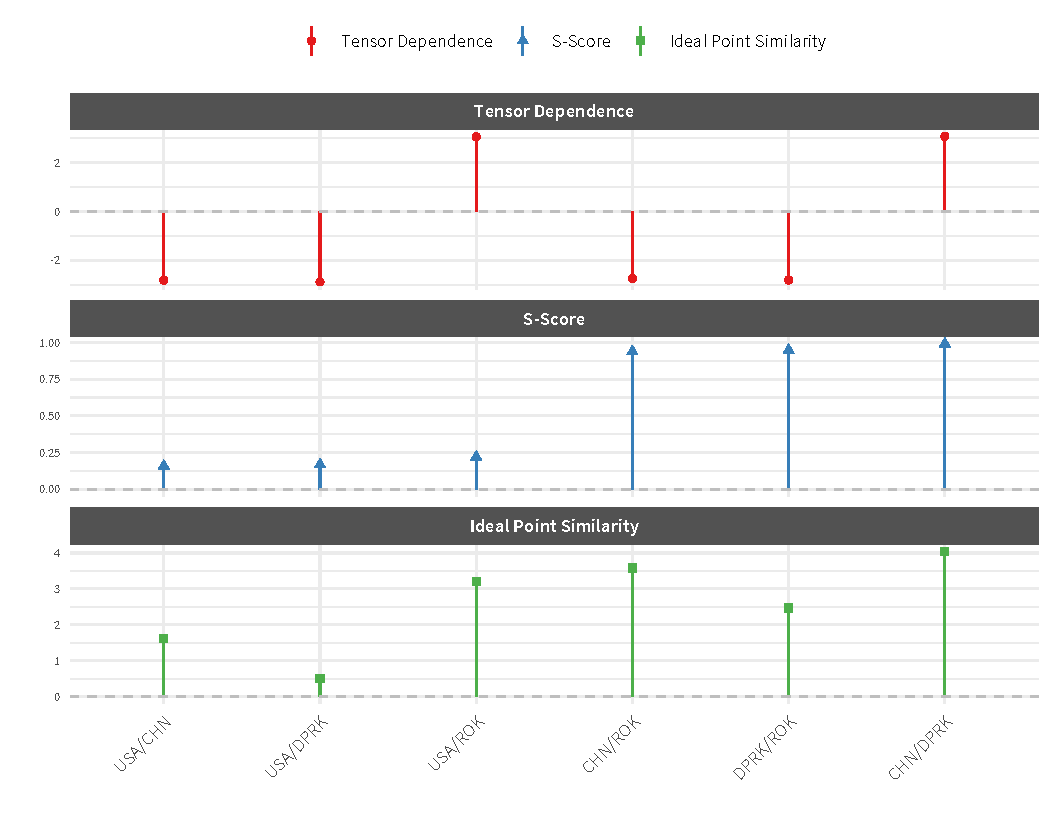
\includegraphics[width=1\textwidth]{idPtScoreLatAngleViz}
\caption{Visualization of tensor dependence, S-score, and ideal point similarity relationships between China (CHN), North Korea (DPRK), South Korea (ROK), and the United States (USA) in 2012. Within each panel a higher score denotes that the countries have a more positive relationship.}
\label{korea:withus}
\end{figure}

To generalize this test of face plausibility, we present all three measures' accounts of six dyadic relationships over time. In each of the plots, we have standardized each of the measures and higher scores denotes that countries have a more positive relationship. We first look at three close relationships where we would expect to see similar preferences. Figure \ref{friendly:dyads} depicts the relationships between France and Germany, the US and Israel, and North Korea and China. In all three cases our tensor dependence measure consistently places each of these relationships on the positive end of the spectrum. S-Scores correctly classify Franco-German and Sino-North Korean friendship, while the US/Israel relationship is characterized as actually quite poor. The ideal points similarity measure largely matches what we find with tensor dependence but shows notably more variation in the quality of these relationships over time.

\begin{figure}
	\centering
	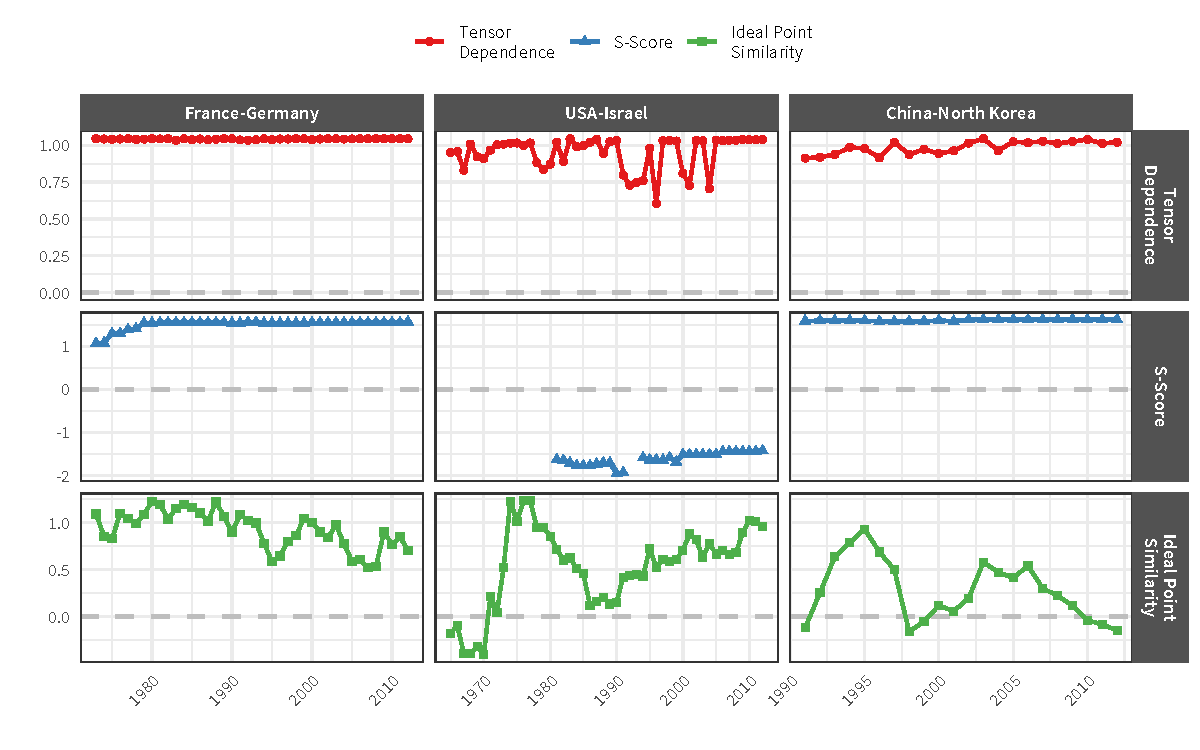
\includegraphics[width=1\textwidth]{plausPlot_1_border}
	\caption{Dyadic relationships between France-Germany, United States-Israel, and China-North Korea according to the different preference measures. Yearly tensor dependence scores between dyads are denoted by red circles, ideal point similarity based on UN voting in blue triangles, and S-scores by green squares. Each of the measures is standardized and within each panel a higher score denotes that the countries have a more positive relationship. The grey dashed line in each of the panels designates a neutral relationship.}
	\label{friendly:dyads}
\end{figure}

In Figure \ref{unfriendly:dyads} we look at the United States' relationship with three countries that are characterized by change and major events. S-scores are the only measure that do not detect a marked improvement in the US/Russian relationship at the end of the Cold War. Both the UN ideal points and tensor dependence measures find significant improvements followed by a drift toward enmity, whereas S-scores have a constant (though slightly improving) neutral relationship. The tensor dependence measure also shows that the US-Russia relationship in the years immediately after the Cold War was actually quite positive. Additionally, the tensor dependence measure for US and Russia does spike in 2010 likely because of Russia joining the US and its allies in placing tighter sanctions on Iran. For the US and Iraq no measure depicts more similar preferences following the US occupation, though only our tensor dependence measure finds a substantial increase in enmity in the run-up to the United States' 2003 invasion. Finally, each of the measures do find that the US relationship with China is quite weak.

\begin{figure}
	\centering
	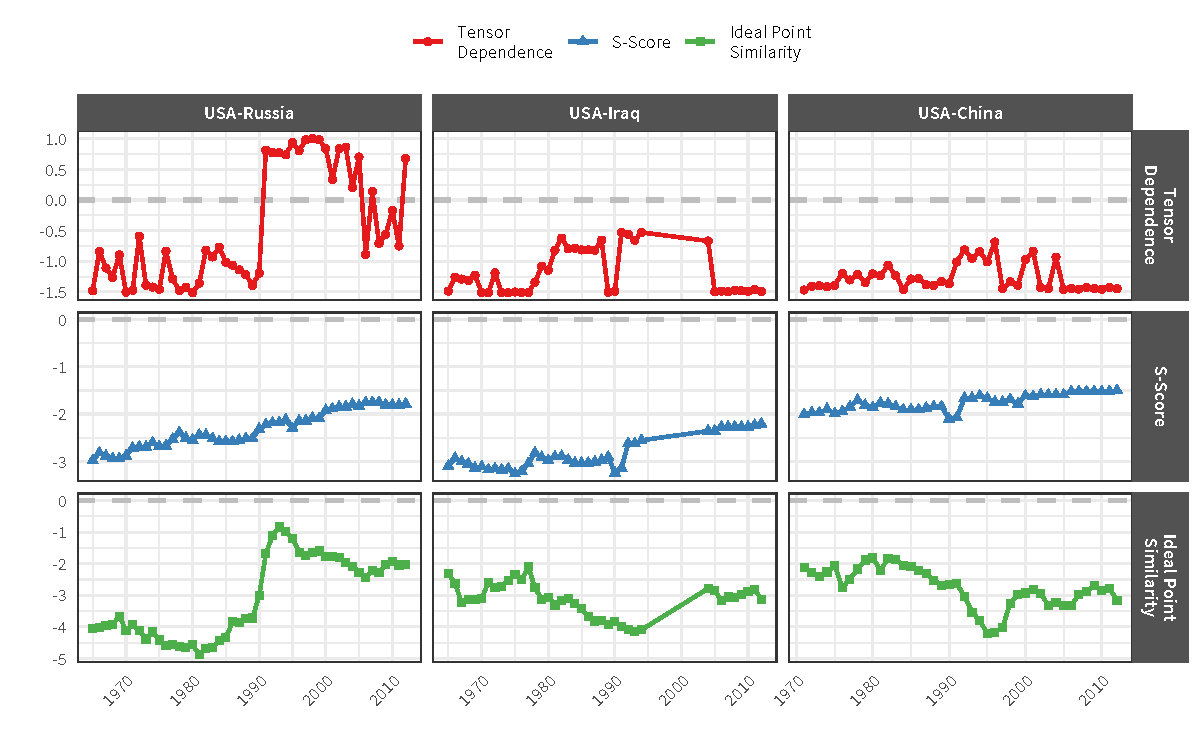
\includegraphics[width=1\textwidth]{plausPlot_2_border}
	\caption{Dyadic relationships between France-Germany, United States-Israel, and China-North Korea according to the different preference measures. Yearly tensor dependence scores between dyads are denoted by red circles, ideal point similarity based on UN voting in blue triangles, and S-scores by green squares. Each of the measures is standardized and within each panel a higher score denotes that the countries have a more positive relationship. The grey dashed line in each of the panels designates a neutral relationship.}
	\label{unfriendly:dyads}
\end{figure}

As can be seen from these relationships, the measure of preferences based on tensor dependence distance is in many cases as plausible or more than incumbent measures of preferences. While the measure has more temporal instability than S-scores or UN ideal points, in these six cases it often does better, and rarely worse at conforming to our expectations of the relationships. Of course, this could just be a case of us picking particularly propitious cases.

\subsection*{Relationship between Tensor Dependence and Components}

We also examine how our tensor dependence measure is affected by changes in alliance relations or UN voting similarity by considering the relationship between the United States and Israel in 1981. With the signing of the ``Joint Memorandum of Understanding," the two states went from having no alliance relationship to having one, the states were voting together at the UN 80\% of the time (up 3\% from 1980, below the median yearly change for this dyad). These factors, coupled with changes in the third order effects for the dyad, led the tensor dependence to increase from about 2.72 to about 3.08.

Of course, another pair of countries might sign an alliance (or withdraw from an alliance) and have a markedly different effect on this measure of tensor dependency. For example, in 1977, the United Kingdom and the United States went from being in 5 alliances together to being in 4, and this led to a drop in their tensor dependence from 3.13 to 2.28, despite a decrease in their UN voting similarity of less than 1\%. This is because the alliance that ended in 1977 was the Southeast Asian Treaty Organization, which had 4 other members, and so the third order effects were concomittantly more severe. To capture the aggregate effects of dyadic variables on our measure of tensor dependence, we estimate a simple AR(1) model, depicted in Table~\ref{tensor:ols}, and these dyadic factors account for about 78\% of the variance, with the rest coming from third order factors. Next, we conduct a the large-N analysis of conflict and compare the added utility of these various measures of state preferences.

\begin{table}[ht]
	\centering
	\begin{tabular}{lcccc}
		\hline
		& Estimate & Std. Error & t value & Pr($>|t|$) \\
		\hline
		(Intercept) & 0.0773 & 0.001 & 74.26 & 0.000 \\
		Tensor Dependence$_{t-1}$ & 0.888 & 0.0004 & 2094.81 & 0.000 \\
		Change in Alliance Relationship & 0.131 & 0.009 & 15.30 & 0.000 \\
		Change in UN Voting Similarity & 4.401 & 0.014 & 313.14 & 0.000 \\
		\hline
	\end{tabular}
	\caption{Regression of tensor dependence on dyadic components.}
	\label{tensor:ols}
\end{table}

\subsection*{Model Competition}

To evaluate the different measures of state preference similarity, we assess their utility in predicting the occurrence of interstate disputes. Here we look at four non-nested models: a model using no measures of state preferences, one using an S-Score based on similarity in alliance portfolio \citep{signorino:ritter:1999}, one using the ideal points determined by UN voting \citep{bailey:etal:2015}, a model using both UN ideal points and alliance S-scores, and finally, a model using our tensor dependence approach that combines the raw data from UN voting and alliances. We evaluate the models on two criteria: whether state preference similarity have a consistent effect in the predicted direction, and how well each model does at predicting disputes in an out-of-sample context.

In each of these models, we utilize a logistic regression of Militarized Interstate Dispute (MID) participation on measures of state preferences and a vector of control variables. These control variables overlap with the standard framework used in O'Neal and Russett's canonical work on the democratic peace \citep{oneal:russett:1997}.\footnote{The exception is that our models ignore trade interdependency, as including that data drastically decreases the number of observations.} In particular, we include a binary measure of joint democracy (whether both states have Polity IV scores $\geq 7$), whether the states are contiguous, and the ratio of state capabilities as measured by the Correlates of War Project's Composite Index of National Capabilities (CINC). We also account for temporal interdependence using a peace year spline \citep{carter:signorino:2010}.

\subsection*{In-sample explanation}

As detailed in figure \ref{fig:coefP}, two of the measures of state preference similarity perform as we would expect.\footnote{Given that our estimate of $\bl A$ comes with uncertainty, we also ran our analysis using several different draws from the distribution for $\bl A$, when combining these estimates via \citet{rubin:1976}'s rules, we found results similar to what is shown below.}  Our measure of state preference using tensor dependence difference is significant and negative: states that are more similar to one another based on our measure are less likely to engage in conflict. Similarly, UN ideal point similarity passes this test. The measure using UN voting ideal points is negative and clearly distinct from $0$, indicating that states with higher levels of similarity in terms of UN voting are less likely to find themselves in conflict. On the other hand, higher alliance S-scores are consistently associated with higher probabilities of conflict -- so states with more similar preferences as measured using alliance portfolios are more likely to quarrel. This is, to say the least, surprising. These results hold when those measures of preference are used in isolation, or in tandem. The effects of the control variables are consistent when using differing versions of state preference and also generally align with the extant literature.

\begin{figure}[ht]
	\centering
	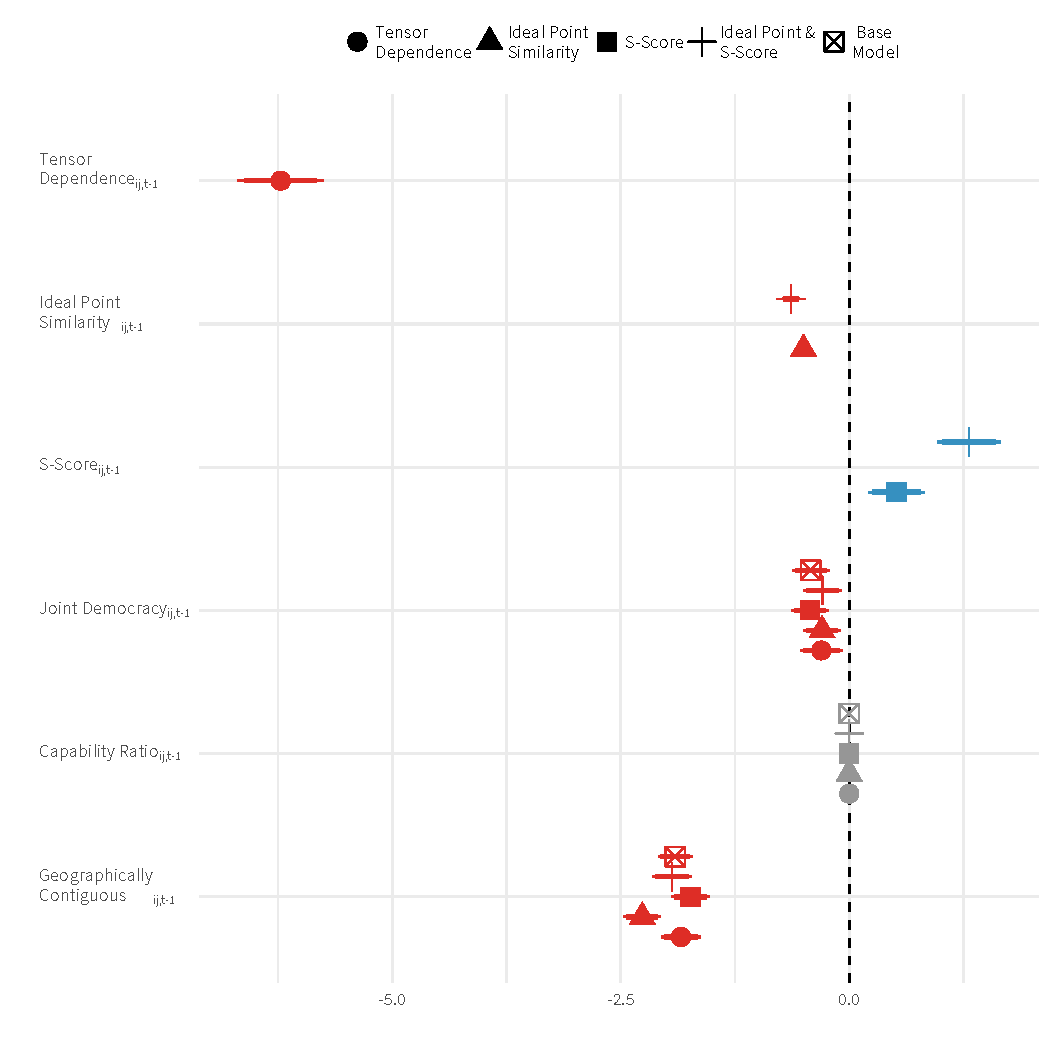
\includegraphics[width=.7\textwidth]{betaEst}
	\caption{Parameter estimates from models with different measures of state preference. Point represents average estimate, line through the point represents the 95\% confidence interval.}
	\label{fig:coefP}
\end{figure}
\FloatBarrier

\subsection*{Out-of-sample prediction}

Given these results, we can say that two of the measures of preferences behave as we would expect, while S-scores do not. To adjudicate between the two measures of preference similarity that pass this test, and help determine what we should make of the differing effect of democracy, we turn to out-of-sample prediction. We undertake a cross-validation procedure in which we partition our data into 30 different folds. This process works by taking each fold, $k$, and running a logistic model excluding data from that fold. Once we have parameter estimates from a model that excluded fold $k$, we predict the probability of a MID in fold $k$ using only the parameter estimates and the covariates from fold $k$.

We then compare the performance of these models using two metrics: area under the Receiver Operator Characteristic Curve (AUC-ROC) and the Precision Recall Curve (AUC-PR). The ROC curve examines the tradeoff between true positives and false positives, and the PR examines the tradeoff between making only correct predictions and predicting all the disputes that occurred. In general, the ROC will disproportionately reward those models that predict $0$ well -- and we can interpret the ROC as the likelihood a prediction is correct. The numeric value for the PR has less of a clear interpretation, but models with a higher PR do a better job of predicting when events actually occur.

As shown in figure \ref{fig:roc}, the model using tensor dependence distance decisively outperforms the other models. While the AUC-ROC is somewhat higher with the tensor dependence model, the real difference between the measures shines through in the AUC-PR, where the model using this measure performs almost twice as well as the base model. In contrast, models using other measures of state preferences yield only minimal improvements in prediction over the base model. This is especially relevant because AUC-PR specifically focuses on the difficult task of predicting conflict, compared to the relatively easier task of predicting non-conflict that is rewarded by the AUC-ROC measure.

\begin{figure}[ht]
	\centering
	\begin{tabular}{cc}
	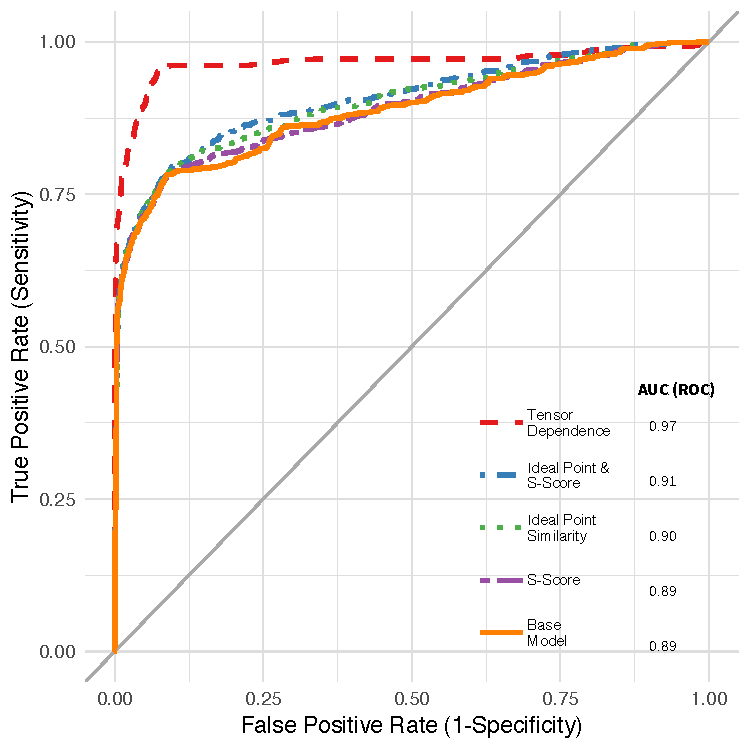
\includegraphics[width=.4\textwidth]{roc_outSample} &
	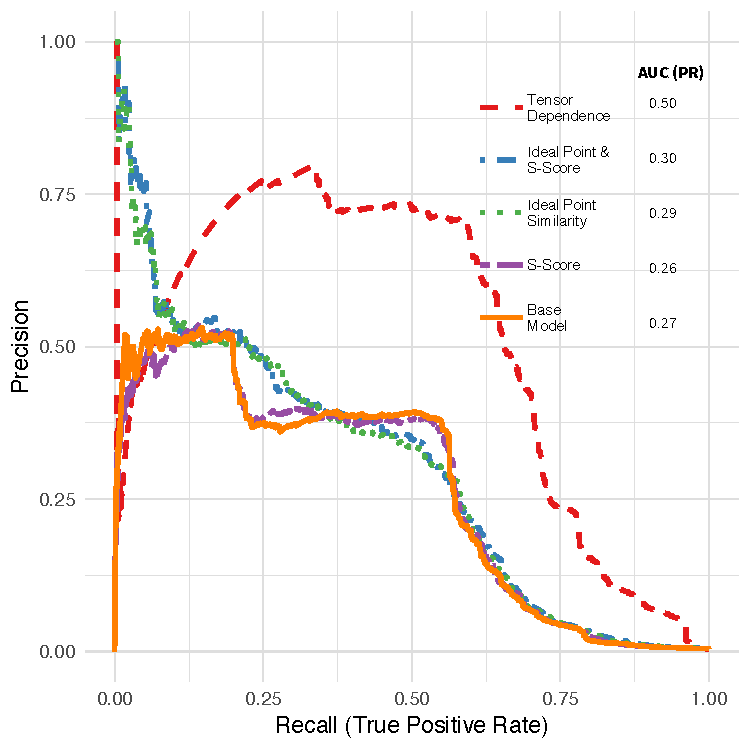
\includegraphics[width=.4\textwidth]{rocPr_outSample}
	\end{tabular}
	\caption{Assessments of out-of-sample predictive performance using ROC curves and PR curves. AUC statistics are provided as well for both curves.}
	\label{fig:roc}
\end{figure}
\FloatBarrier

In addition, to this cross-validation test we also include a forecasting exercise. Specifically, we repeatedly estimate our model using three years of data and forecast the next year. Our sample ranges from 1966 to 2008, so we estimate a model using data from 1966 to 1968 and then predict conflicts in 1969. Next, we train a model using data from 1967 to 1969 and predict conflicts in 1970. We repeat this iteratively for all years using a three year rolling window, until we have generaed out of sample predictions for every year in our sample from 1969 to 2008. We depict the performance results from this analysis below in Figure~\ref{fig:rocTime}. The results that we get from this forecasting exercise are similar to those via the 30-fold cross-validation, and provide further reason for confidence in the usefulness of this measure of state preferences.

\begin{figure}[ht]
	\centering
	\begin{tabular}{cc}
	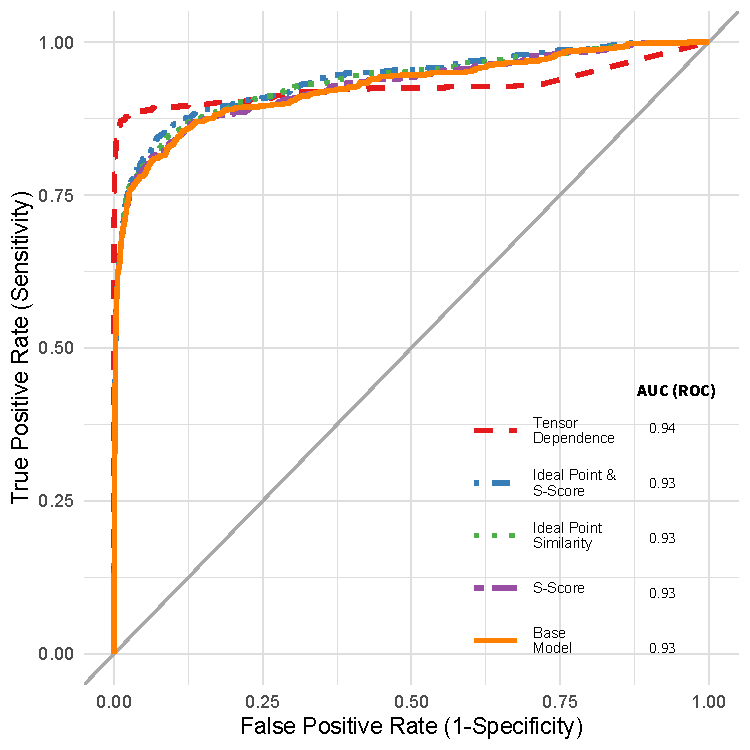
\includegraphics[width=.4\textwidth]{roc_outSample_time2} &
	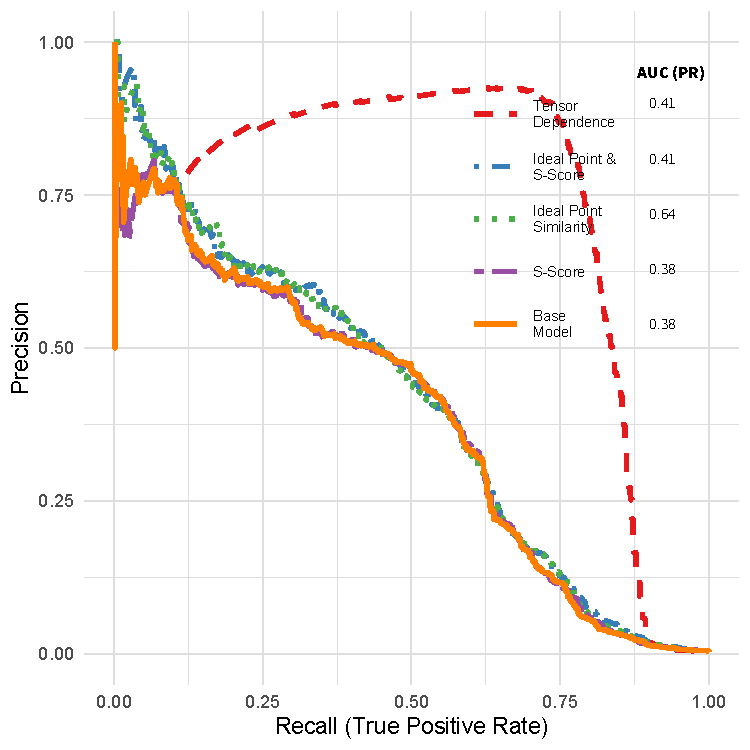
\includegraphics[width=.4\textwidth]{rocPr_outSample_time2}
	\end{tabular}
	\caption{Forecasting assessments of out-of-sample predictive performance using ROC curves and PR curves. AUC statistics are provided as well for both curves.}
	\label{fig:rocTime}
\end{figure}
\FloatBarrier

\section*{Conclusion}

We use a network methodology to create a new measure of state preference similarity using both UN Voting and alliance data. This measure of preference similarity demonstrates face plausibility comparable or superior to existing measures when it comes to capturing the dynamics of a number of notable dyadic relationships.\footnote{There is an important limitation to keep in mind with the measure that we have generated, namely that we run separate models with a fixed three year rolling temporal window to estimate this measure. In future work, exploring the value-add from employing a single model that can generate time varying measures of state preference from multiple dimensions of state relations over time would likely be of notable value. A number of works have explored measuring low-dimensional relationships between actors using dynamic latent space models (e.g., \citealp{sewell:chen:2015}), and that work will certainly prove to be informative in future work that seeks to extend these ideas to the tensor setting.}  We then attempt to use this measure of state preferences in a predictive model of interstate disputes. In doing so, we find that the measure of preferences has the expected effect (states with similar preferences are less likely to be involved in disputes). Most importantly, a model of interstate conflict that includes our measure of preference similarity decisively outperforms models that include both of the most prominent existing measures of preferences.

While this measure of state preference similarity has yielded leverage in predicting conflict, it should also be useful in answering a number of other questions. One possible use would be to look at the measure of state preferences as an outcome variable, rather than a predictor. We could here look at how preferences change in tandem with leadership change -- can we find evidence, for example, that the election of Donald Trump moved the United States' foreign policy preferences away from the major Western European states and towards Russia's? We could also see how well this measure of state preference similarity predicts more collaborative behavior -- treaty membership or trade for example.

Ours is not the first paper to use network analysis to attempt to measure a theoretically important but difficult to observe phenomenon. For example, \citet{moody:white:2003} measured social cohesion by looking at the minimum number of paths connecting each actor in a group (and applied to high school friendship networks and among American businesses. \citet{beardsley:etal:2018} generates a measure of hierarchy by looking at a network of arms transfers and first finding the clusters in each group,  then how central an actor is within a given cluster, they go on to use this measure of hierarchy in a downstream model to explain interstate conflict, and similarly \citet{cranmer:etal:2015} use a measure of multiplex modularity in the network of alliances, trade, and international organization membership to measure ``Kantian fractionalization"--the extent to which the international system is fragmented between liberal and illiberal states.

In addition to helping us to understand state preferences, this sort of technique could help in measuring phenomena like social cohesion and hierarchy, or spatial contagion. If one wanted to use network approach to measure social cohesion, one could potentially do this with a Latent Class Model as in \citet{airoldi:etal:2008}. Using some measure of social interaction, this model would give the probability that each member is in a particular clique or subgroup in society. We could then look at how many members of society have probability of membership in multiple groups above a certain threshold to see how many individuals bridge different groups, contributing to our understanding of social cohesion. In understanding how phenomenon -- violence, diseases, new technology to name a few examples -- diffuse, many scholars rely on spatial lag models, which require the scholar to specify a spatial weights matrix that indicates how likely a phenomenon is to move from one area to another. Of course, we can never know the true adjacency matrix, and so scholars use a proxy, most often some form of geographic distance. We may be able to improve the predictive performance of spatial models by inferring a weights matrix using a network approach based on how the phenomenon has diffused in the past.

In general, there are a wide variety of substantive areas in which using network models to extract measurements of how actors relate may provide new insights. We would certainly not argue that the approach we present here can easily be plugged into alternative applications.\footnote{\citet{goldenberg:etal:2010} and \citet{kim:etal:2018} provide helpful discussions of various types of network models that have emerged to study cross-sectional and multilayer networks.} In fact, despite the benefits we highlighted of our approach for measuring state preferences, there are downsides. Most notably, our choice of manually choosing the last three years of data could certainly be iterated on in future research. \citet{park:sohn:2017}, for example, present a model to actually determine when there are discrete changes in the underlying group structure of network entities. In future research, further exploring how network models can be used to address measurement problems may prove to be a fruitful area of research.

\newpage

\section*{Conflicts of Interest}

Authors have nothing to disclose.

% Bib stuff
\clearpage
% \bibliography{C:/Users/herme/whistle/master}
% \bibliography{C:/Users/Owner/whistle/master}
% \bibliography{C:/Users/maxgallop/Documents/whistle/master}
\bibliography{C:/Users/S7M/whistle/master}
% \bibliography{/Users/s7m/whistle/master}
\bibliographystyle{elsarticle-harv}\biboptions{authoryear}

\end{document}
